\begin{pastexam}[label={px:gw3-113-ds-03}]{關務三等資訊處理 113 年 第三題}
（申論；25 分）

有一棵高度平衡二元搜尋樹（balanced binary search tree）又稱 AVL 樹（Adelson-Velskii Landis tree）如下圖，加入 90，請詳細
說明該如何調整成一棵 AVL 樹？接著再加入 85，請詳細說明該如何調整成一棵 AVL 樹？接著再刪除 15，該如何調整成一棵 AVL 樹？
請將最後調整後的 AVL 樹中每個節點之平衡因子（balance factor）寫在節點旁邊。（25 分）
\begin{center}
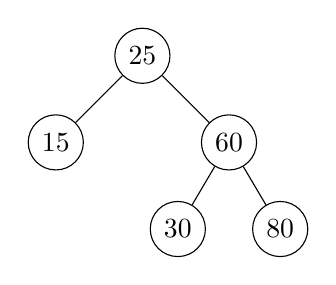
\begin{tikzpicture}[every node/.style={circle,draw,minimum size=7mm,inner sep=0pt},
  level distance=11mm, level 1/.style={sibling distance=22mm}, level 2/.style={sibling distance=13mm}]
\node {25}
  child {node {15}}
  child {node {60} child {node {30}} child {node {80}}};
\end{tikzpicture}
\end{center}
\end{pastexam}

\begin{pastsoln}
答案：加入 90 後在 25 做 RR 旋轉（左旋）；加入 85 後在 80 做 RL 旋轉；刪除 15 不需調整。 最後的樹是 60(25(\,·\,, 30),
85(80, 90))，平衡因子：60 是 $0$、25 是 $-1$、其餘都是 $0$。

平衡因子 $\mathit{bf}(x) = $ 左子樹高度 $-$ 右子樹高度（空樹高度 $0$，葉子高度 $1$），AVL 樹要求每個節點
$\mathit{bf} \in \{-1, 0, 1\}$（資結書第~10.2~節）。 原來的樹：15、30、80 是 $0$，60 是 $0$，25 是 $1 - 2 = -1$，合格。

\textbf{加入 90。} 照二元搜尋樹插入：$90 > 25$ 往右，$> 60$ 往右，$> 80$，成為 80 的右子節點。 沿路往上更新：
$\mathit{bf}(80) = -1$，$\mathit{bf}(60) = 1 - 2 = -1$，$\mathit{bf}(25) = 1 - 3 = -2$，失衡。 最低的失衡節點是 25，新節點
在 25 的右子樹（60）的右子樹（80）裡，屬於 \textbf{RR 型}，在 25 做一次左旋（資結書第~10.1~節）：60 升為根，25 變成 60
的左子節點，60 原本的左子樹 30 改掛到 25 的右邊。
\begin{center}
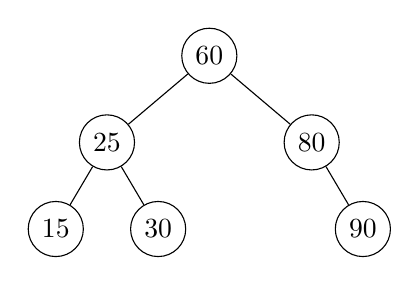
\begin{tikzpicture}[every node/.style={circle,draw,minimum size=7mm,inner sep=0pt},
  level distance=11mm, level 1/.style={sibling distance=26mm}, level 2/.style={sibling distance=13mm}]
\node {60}
  child {node {25} child {node {15}} child {node {30}}}
  child {node {80} child[missing] child {node {90}}};
\end{tikzpicture}
\end{center}
平衡因子：60 是 $2 - 2 = 0$，25 是 $0$，80 是 $-1$，葉子都是 $0$。 樹高從 $3$ 回到 $3$（插入前的高度），上面不必再調整。

\textbf{加入 85。} $85 > 60$ 往右，$> 80$ 往右，$< 90$，成為 90 的左子節點。 往上更新：$\mathit{bf}(90) = 1$，
$\mathit{bf}(80) = 0 - 2 = -2$，失衡。 新節點在 80 的右子樹（90）的\textbf{左}子樹裡，屬於 \textbf{RL 型}，要做雙旋轉：先在 90
右旋、再在 80 左旋，結果 85 升為這棵子樹的根，80 是它的左子節點、90 是右子節點。
\begin{center}
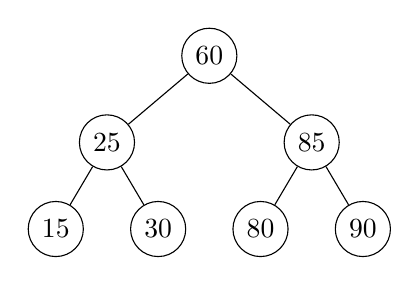
\begin{tikzpicture}[every node/.style={circle,draw,minimum size=7mm,inner sep=0pt},
  level distance=11mm, level 1/.style={sibling distance=26mm}, level 2/.style={sibling distance=13mm}]
\node {60}
  child {node {25} child {node {15}} child {node {30}}}
  child {node {85} child {node {80}} child {node {90}}};
\end{tikzpicture}
\end{center}
子樹高度回到 $2$，60 的平衡因子 $2 - 2 = 0$，全部節點的平衡因子都是 $0$。

\textbf{刪除 15。} 15 是葉子，直接拿掉。 往上更新：$\mathit{bf}(25) = 0 - 1 = -1$，仍合格；25 的高度還是 $2$，所以
$\mathit{bf}(60) = 2 - 2 = 0$。 沒有節點失衡，\textbf{不需要旋轉}。

\textbf{最後的 AVL 樹}（節點旁是平衡因子）：
\begin{center}
\begin{tikzpicture}[every node/.style={circle,draw,minimum size=7mm,inner sep=0pt},
  level distance=12mm, level 1/.style={sibling distance=30mm}, level 2/.style={sibling distance=15mm},
  bf/.style={draw=none,rectangle,font=\small,text=black!70}]
\node (r) {60}
  child {node (a) {25} child[missing] child {node (b) {30}}}
  child {node (c) {85} child {node (d) {80}} child {node (e) {90}}};
\node[bf,right=1mm of r] {$0$};
\node[bf,left=1mm of a] {$-1$};
\node[bf,below=0.5mm of b] {$0$};
\node[bf,right=1mm of c] {$0$};
\node[bf,below=0.5mm of d] {$0$};
\node[bf,below=0.5mm of e] {$0$};
\end{tikzpicture}
\end{center}
中序是 $25, 30, 60, 80, 85, 90$，仍是二元搜尋樹。
\end{pastsoln}
